%%=============================================================================
%% Literatuurstudie
%%=============================================================================

\chapter{Literatuurstudie}
\label{ch:literatuurstudie}

\section{Wat is Android Wear?}
\label{sec:androidwear}
Android Wear is Google's platform voor wearables. Een wearable worden beschreven door \textcite{Dictionary} beschreven als een computer of geavanceerd elektronisch toestel dat geïncorporeerd is in een accessoire gedragen op het lichaam of in een kledingstuk. 
\textcite{Techradar} heeft enkele van de belangrijkste kenmerken van Android Wear opgelijst.
Android Wear is gebouwd voor kleinere toestellen en met hands-free gebruik in het achterhoofd. Het maakt de toegang tot enkele van uw smartphone's makkelijkste functionaliteiten zo makkelijk als naar beneden kijken naar uw pols. Het is vooral bedoeld om de notificaties van uw smartphone makkelijk te weergeven zodat niet elke keer gezocht moet worden naar de smartphone in de broekzak. Gebaseerd op uw Google zoekopdrachten zullen real-time scores van uw favoriete sportteam, verkeerdscondities of afspraken in uw afgenda weergeven worden. Als het Android Wear toestel NFC (Near Field Communication) ingebouwd heeft, kan er in verschillende landen (momenteel Australië, Hong Kong, Ierland, Japan, Nieuw-Zeeland, Polen, Singapore, Verenigd Koninkrijk en de Verenigde Staten volgens de support van \cite{Androidpay}) ook met de wearable betaald worden via Android Pay. Ook spraakherkenning kon niet ontbreken in de Android Software. Door deze technologie kan je de wearable's spraakherkenning activeren door "OKay, Google" te zeggen of door de aanknop ingedrukt te houden. Google Assistant zal u hierop verderhelpen. Android Wear is compatibel met smartphones die draaien op Android 4.3 of hoger en iOS 9 of hoger. Eén van de belangrijkste app categorieën op Android Wear zijn de gezondheidsapps. Hiervoor wordt standaard gebruik gemaakt van Google Fit. Met Google Fit kan je kiezen tussen verschillende workouts tijdens het sporten, of bijvoorbeeld een dagelijks doel instellen voor het aantal stappen dat u wil nemen.  
\begin{figure}[H]
	\centering
	\caption{\textit{Enkele voorbeelden van smartwatches gebruikmakend van Android Wear}}
	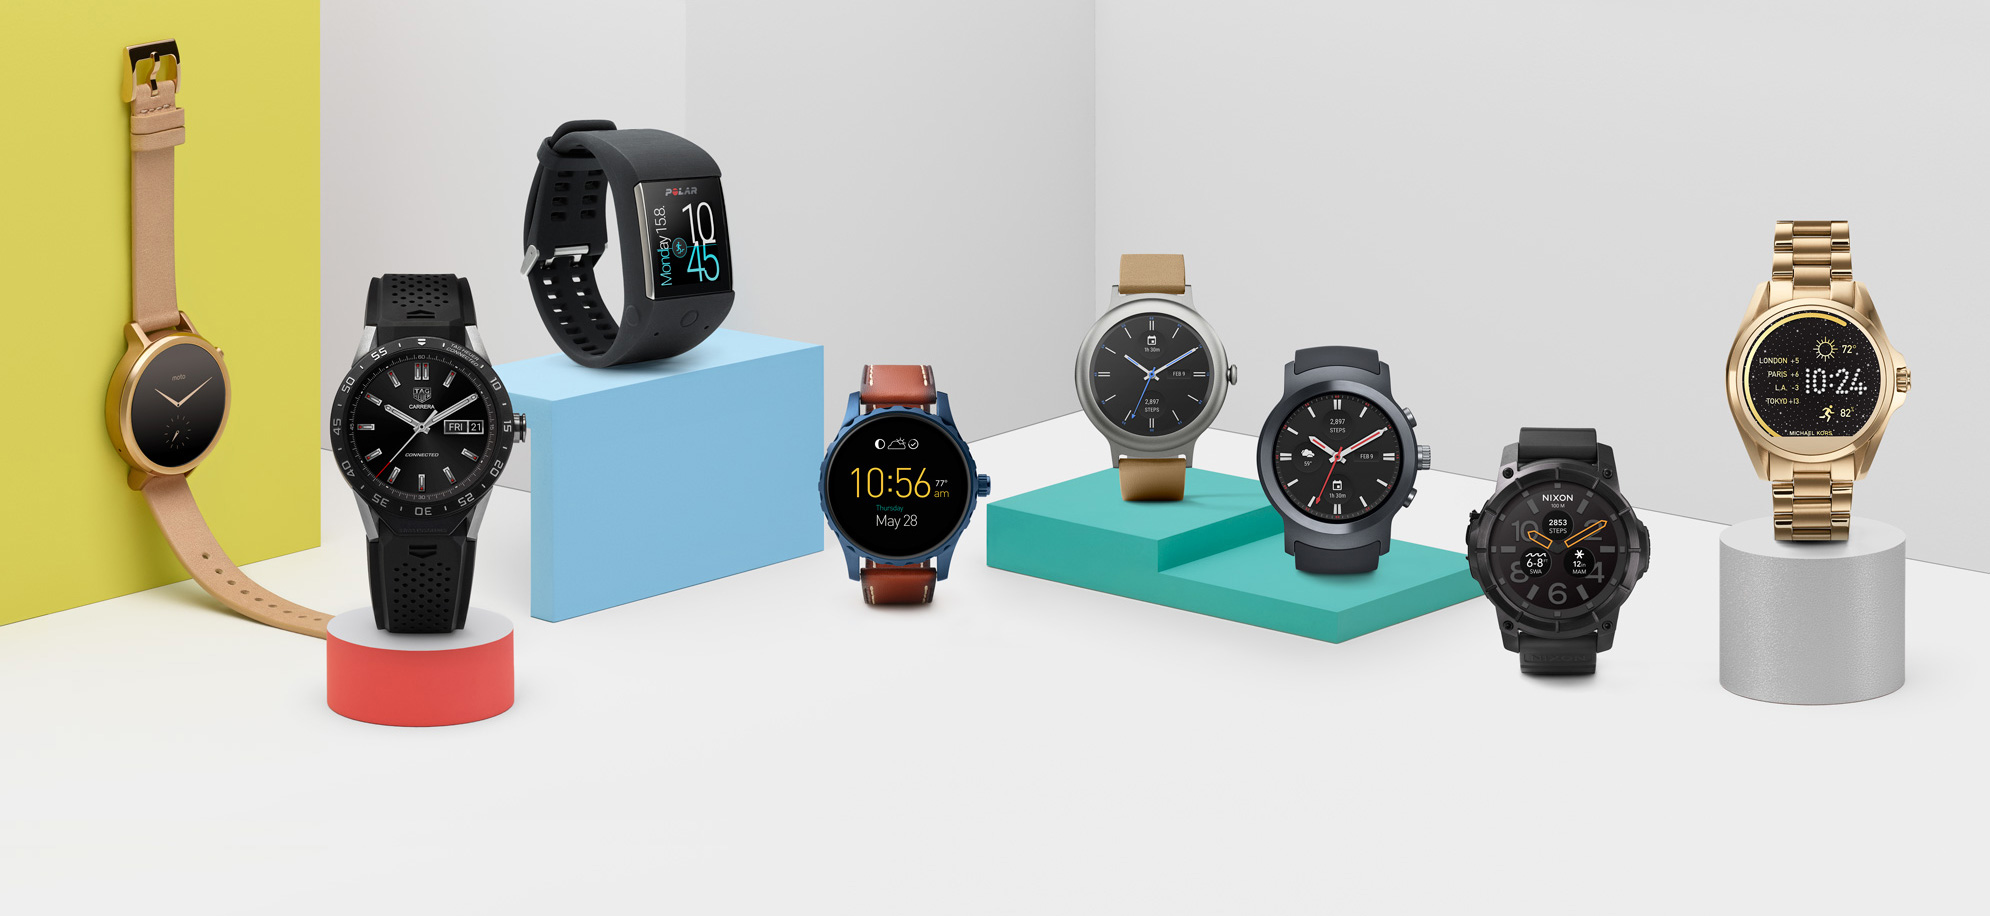
\includegraphics[width=10cm, height=10cm, keepaspectratio]{img/WearExamples}\\[.5cm]
\end{figure}
%% TODO:
%% Uit je probleemstelling moet duidelijk zijn dat je onderzoek een meerwaarde
%% heeft voor een concrete doelgroep (bv. een bedrijf).
%%
%% Wees zo concreet mogelijk bij het formuleren van je
%% onderzoeksvra(a)g(en). Een onderzoeksvraag is trouwens iets waar nog
%% niemand op dit moment een antwoord heeft (voor zover je kan nagaan).
\section{Wat is een APK en uit wat bestaat dit?}
APK staat voor Android Application Package. Volgens \textcite{PCMag} is een APK een applicatie bestand klaar voor installatie op een Android toestel. Het gecompresseerde APK bestand, een ZIP archief in JAR-formaat, wordt gedistribueerd naar Android gebruikers voor de installatie op hun smartphone, tablet of wearable. 
Een APK bestand bestaat normaliter uit volgende elementen : 
\begin{enumerate}
	\setlength\itemsep{2em}
\item \textbf{classes.dex} \newline
Bevat gecompileerde applicatiecode, getransformeerd naar een Dex bytecode. Het is mogelijk dat er meerdere DEX bestanden in de APK staan als er multidex gebruikt wordt om de 65536 limiet te overkomen. Vanaf Android 5.0, met de introductie van ART runtime, worden deze bestanden gecompileerd naar OAT bestanden door de compiler bij de installatie en worden deze op het toestel zijn data partitie geplaatst. 
\item \textbf{res/} \newline
Deze folder bevat de meeste XML bestanden en drawables (bijvoorbeeld PNG of JPEG bestanden) in mappen met verschillende kwalificaties, zoals -mdpi en -hdpi voor schermdichtheden, -sw600dp of -large voor schermgroottes, en -en, -de, -pl voor talen. De XML bestanden worden automatisch gecompileerd naar een compactere binaire representatie, dus deze kunnen niet met een teksteditor geopend worden vanuit de APK. 
\item \textbf{resources.arsc}\newline
Sommige resources en identifiers worden gecompileerd naar dit bestand. Het wordt normaal ongecomprimeerd opgeslagen in de APK voor snellere toegang tijdens runtime. Dit bestand manueel comprimeren kan een makkelijke oplossing lijken, maar dit is geen goed idee door 2 redenen. Eén, Play Store comprimeert alle data voor transfer automatisch en twee, dit bestand comprimeren in de APK verspilt systeem resources (RAM) en performantie (vooral de opstarttijd van de app).
\item \textbf{AndroidManifest.xml}\newline
Gelijklopend met andere XML resources wordt de applicatie Manifest getransformeerd naar een binair formaat tijdens de compilatie. De Play Store gebruikt bepaalde informatie in de AndroidManifest om te bepalen of een APK kan geïnstalleerd worden op een bepaald toestel, zo zijn er controles op toegelaten schermdichtheden of schermgroottes, beschikbare hardware en kenmerken (bijvoorbeeld aanwezigheid van een touchscreen). Deze Manifest inhoud kan geïnspecteerd worden na compilatie, gebruik hiervoor de aapt tool van de Android SDK: 
\begin{lstlisting}[backgroundcolor = \color{lightgray}, xleftmargin = 2cm,
framexleftmargin = 1em]
$ aapt dump badging your_app.apk
\end{lstlisting}
\item \textbf{libs/}\newline
Alle native libraries (*.so bestanden) zullen in submappen geplaatst worden genaamd naar de ABI (CPU architectuur, bv. x86, \texttt{x86\_64}, armeabi-v7a) die ze als doel hebben onder de libs/ map. Normaal worden deze uit de APK gekopieerd naar de datapartitie tijdens het installeren van de applicatie. Echter, sinds de APK zelf nooit aangepast wordt zolang deze op het toestel van de gebruiker staat, neemt dit dubbel zoveel plaats in voor elke native library. 
\item \textbf{assets/}\newline
Deze map zal gebruikt worden voor alle bestandonderdelen die niet als Android-type resources gebruikt zullen worden. Meestal zullen dit lettertypebestanden of game data zijn, zoals levels of textures, samen met andere applicatiedata die direct geopend moet kunnen worden als een file stream.
\item \textbf{META-INF/}\newline
Deze map is aanwezig in ondertekende APKs en bevat een lijst van alle bestanden in de APK met hun handtekening. Momenteel werkt het ondertekenen van bestanden in Android door het verifiëren van de handtekening tegen de ongecomprimeerde bestandinhoud van het archief, één voor één. Dit heeft enkele interessante gevolgen. Doordat elke onderdeel van een ZIP bestand apart opgeslagen wordt, betekent dit dat je individuele bestanden hun compressieniveau kan aanpassen zonder ze opnieuw te ondertekenen. De verificatie van de handtekening zal echter falen wanneer een bestand verwijderd wordt uit het archief nadat het ondertekend werd. 
\end{enumerate}

\begin{figure}[H]
	\centering
	\caption{\textit{De structuur van de APK}}
	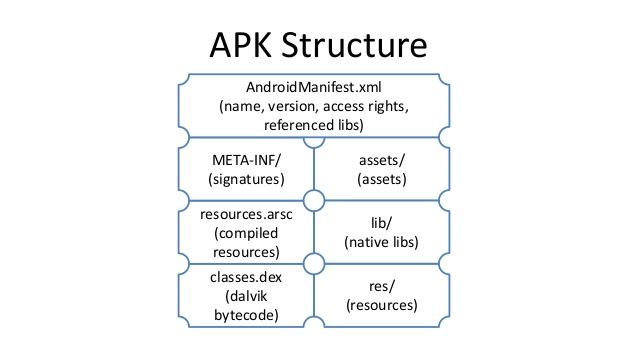
\includegraphics[width=10cm, height=10cm, keepaspectratio]{img/ApkStructure}\\[.5cm]
	
\end{figure}

\section{Verschillende compressietechnieken}
\label{sec:compressietechnieken}

\subsubsection{Technieken gebruikt bij Cozmos, app-ontwikkelaar van Android (Wear) apps}
Bij Cozmos is de belangrijkste tool die gebruikt wordt om de APK zo klein mogelijk te houden Proguard. Proguard zorgt er niet enkel voor dat je code moeilijker leesbaar wordt bij reverse engineering maar het verwijdert ook al je ongebruikte code en resources.
Bij de grotere klanten waar ook security van groot belang is maken we gebruik van Dexguard. Dexguard is de commerciële variant van Proguard en gaat een stap verder met zijn compressietechnieken maar biedt daarnaast ook tal van andere features aan zoals bescherming van de APK of SDK (Software Development Kit) tegen het klonen ervan, piraterij en extractie van sleutelwaarden uit de APK door gebruik te maken van verschillende encryptie- en obfuscatietechnieken. Anderzijds beschermt Dexguard ook bescherming tegen Dynamic Analysis, zodat er tijdens dat de app actief is geen aanpassingen kunnen gebeuren door omgevings- en certificaatcontroles. 

Eén van de andere manieren om de grootte van de APK te beperken die gebruikt wordt bij Cozmos is kijken naar de manier waarop images en andere resources gebruikt worden. Er kan al ruimte bespaard worden door een juiste keuze te maken tussen jpg/png en verdere compressie toe te passen. Soms is ook geen volledige image nodig maar kan er geopteerd worden voor een 9-patch image of om een drawable in XML te definieren. Bij animaties kan je dan weer het aantal frames gaan beperken.

Bij het gebruik van libraries kan het handig zijn om enkel de modules in het project te importeren die ook daadwerkelijk nodig zijn. Ook worden verschillende libraries tegenover elkaar afgewogen en wordt gekeken welke de laagste method count hebben, het best met het geheugen omgaan, het minste plaats innemen.. Stel dat men een library aan het project zou willen toevoegen om images in te laden dan zou de afweging kunnen gemaakt worden tussen Glide en Picasso. Picasso is 3,5 keer kleiner dan Glide maar anderzijds gebruikt Glide een pak minder geheugen om een image weer te geven. Daar moet dus een afweging gemaakt worden waar de focus ligt voor de app, meer vrije opslagruimte of meer vrij geheugen.

Een andere optie is om niet-essentiële zaken achterwege te laten uit je APK. Afbeeldingen of data die maar voor een beperkte groep gebruikers van belang zijn kunnen beter in realtime gedownload worden in plaats van deze al in de APK te voorzien.

Verder kan er door middel van code zuiniger omgesprongen worden met opslagruimte. Zo dienen enums vermeden te worden, kan je (eenvoudige) afbeeldingen renderen..

Uit de richtlijnen van \cite{googlereduceapksize} voor het verkleinen van de grootte van de APK werden volgende technieken gekozen om te onderzoeken: 

\subsubsection{Verwijder ongebruikte resources}
\label{sec:removeunusedresources}
De ingebouwde lint tool in Android Studio, een statische code analyzer, detecteert resources in de res/ map die in de code niet gerefereerd worden. Android Studio zal hiervan een melding maken, maar zal deze niet automatisch verwijderen. Libraries die u toevoegt kunnen ongebruikte resources meebrengen. Gradle kan deze automatisch verwijderen als "shrinkResources" in de build.gradle wordt toegevoegd. 

\subsubsection{Verklein resource gebruik van libraries}
\label{sec:minimizeresourceslibraries}
Wanneer u een Android app ontwikkelt, worden vaak externe librbaries gebruikt om de gebruiksvriendelijkheid te verhogen. Deze libraries bevatten vaak elementen die voor desktops of servers bedoeld zijn, deze elementen kunnen uit de libraries verwijderd worden indien de licentie dit toestaat.

\subsubsection{Ondersteun enkele specifieke schermdichtheden }
\label{sec:supportspecificdensities}
Vanaf Android 4.4 worden verschillende schermdichtheden ondersteund (ldpi, mdpi, tvdpi, hdpi, xhdpi, xxhdpi en xxxhdpi). Het is niet nodig om elke afbeelding te exporteren naar elke dichtheid. Android zal automatisch de afbeelding schalen naar andere schermdichtheden als er geen specifieke export voorzien is. 

\subsubsection{Verminder animatie frames }
\label{sec:reduceanimationframes}
Voor elke frame in een animatie wordt een aparte afbeelding opgeslaan. Als er bijvoorbeeld een animatie aanwezig is met 30 FPS (frames per second) zullen er 30 afbeeldingen opgeslagen worden, maar vaak is bijvoorbeeld 15 FPS meer dan voldoende, en wordt dus de helft van de ingenomen opslagruimte gebruikt.
\begin{figure}[H]
	\centering
	\caption{\textit{Door vermindering FPS zullen minder aparte afbeeldingen per animatie opgeslagen worden}\newline}
	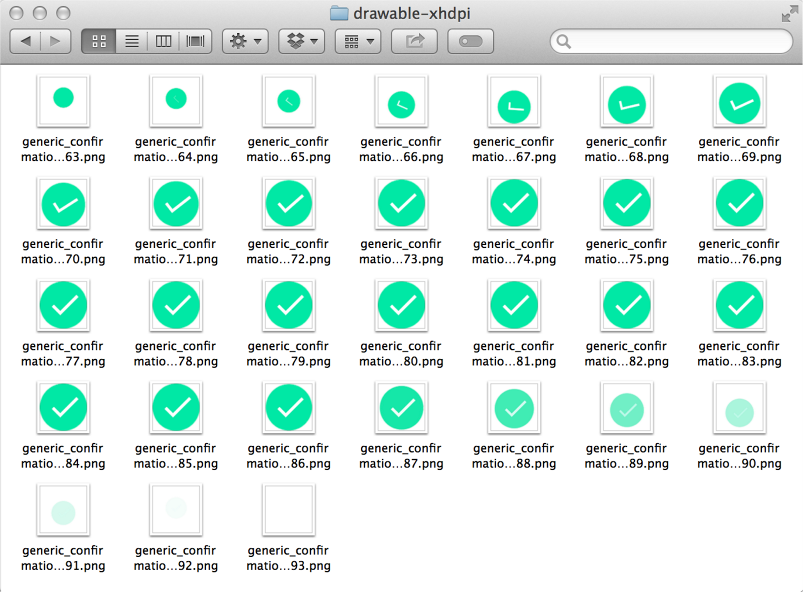
\includegraphics[width=10cm, height=10cm, keepaspectratio]{img/animation-frames}\\[.5cm]
	
\end{figure}
\subsubsection{Hergebruik resources }
\label{sec:reuseresources}
Het is mogelijk om voor elke variatie op een afbeelding (getint, met schaduw of geroteerd) een aparte resource op te slaan. Google raadt echter aan om 1 afbeelding te voorzien, en deze dynamisch tijdens runtime aan te passen. 
Android voorziet verschillende utiliteiten om de kleur van een afbeelding aan te passen.
\subsubsection{Comprimeer afbeeldingen }
\label{sec:compressimages}
De aapt tool kan de afbeelding resources in res/drawable/ optimaliseren met lossless compressie. De tool kan bijvoorbeeld een true-color PNG bestand dat niet meer dan 256 kleuren bevat omzetten naar een 8-bit PNG met een kleurenpallet. Dit resulteert in een afbeelding van eenzelfde kwaliteit maar met een kleinere geheugenvoetafdruk. Deze tool kan geen PNG bestanden in de asset/ folder verkleinen. 

\subsubsection{Gebruik WebP bestandformaat }
\label{sec:webp}
In plaats van PNG of JPEG bestanden, kan er ook gebruik gemaakt worden van het WebP formaat voor afbeeldingen. Dit formaat voorziet lossless compressie (zoals JPEG) en transparantie (zoals PNG) maar voorziet betere compressie dan beide andere formaten. Het gebruik van WebP heeft echter ook enkele nadelen. WebP-ondersteuning is niet beschikbaar bij versies lager dan Android 3.2 (API level 13). Het neemt ook een langere tijd voor het systeem om WebP bestanden te decoderen dan PNG bestanden. Bestaande BPM, JPG, PNG of statische GIF afbeeldingen kunnen naar het WebP formaat omgezet worden door Android Studio. 

\subsubsection{Gebruik vector graphics }
\label{sec:vectorgraphics}
Vector graphics kunnen gebruikt worden om resolutie-onafhankelijke iconen of andere schaalbare media te creëren. Deze afbeeldingen worden in Android gerepresenteerd als VectorDrawable objecten. Met een VectorDrawable object kan een 100-byte bestand een scherpe afbeeldingen genereren op de grootte van het scherm. 
Echter, het neemt a significante tijd voor het systeem om elk VectorDrawable object te genereren. Grote afbeeldingen kunnen zelfs nog langer nemen om op het scherm te verschijnen. Daarom wordt aangeraden de VectorDrawable objecten enkel voor kleine afbeeldingen te gebruiken. 
\subsection{Verminder gebruik code}
\label{sec:reducecode}

\subsubsection{Verwijder automatisch gegenereerde code}
\label{sec:reducegeneratedcode}
Zorg dat u verstaat wat elke lijn gegenereerde code inhoudt, en wat de voetafdruk ervan is. Zo zullen veel protocol buffer tools een groot aantal methodes en klassen genereren, die de grootte van de app kunnen verdubbelen of verdriedubbelen.

\subsubsection*{Verwijder enumeraties}
\label{sec:removeenumerations}
Elke enum kan 1 tot 1.4 KB grootte toevoegen aan uw app's classes.dex bestand. Deze toevoegingen kunnen snel oplopen voor complexe systemen of gedeelde libraries. Indien mogelijk gebruikt u best de @IntDef annotatie en ProGuard om enumeraties te strippen en om te zetten in integers. Deze conversie behoudt alle voordelen van enums. 
\subsubsection*{Verklein grootte native binaries}
\label{sec:reducesizenativebinaries}
Bij het gebruik van native code en de Android NDK (Native Development Kit, hierdoor kan je bepaalde delen van je app implementeren in native-code talen zoals C of C++) kan je de grootte van de app verkleinen door het optimaliseren van de code. Hiervoor zijn 2 technieken bruikbaar :
1) Debug symbolen verwijderen
Wanneer de app niet meer in development is, zijn debug symbolen overbodig. Deze kan je uit de applicatie verwijderen door de "arm-eabi-strip" tool te gebruiken, deze zit ingebakken in Android NDK.
2) Vermijd het extraheren van native libraries
Bewaar .so bestanden ongecompresseerd in de APK, and stel de "android:extractNativeLibs" vlag op false in het "<application>" element van je app manifest. Dit zal vermijden dat de PackageManager de .so bestanden uit de APK naar het bestandssysteem zal kopiëren tijdens de installatie, en zal als bijkomend voordeel hebben dat delta updates van de app kleiner zullen zijn. 
\subsection{Voorzie meerdere APK's}
\label{sec:multipleapks}
De app kan inhoud bevatten die gebruikers downloaden maar nooit gebruiken, zoals regio- of taalgerelateerde informatie. Om een minimale download voor de gebruikers te voorzien, kan de app gesegmenteerd worden in verschillende APKs, gedifferentieerd door factoren zoals schermgrootte of GPU structuur.
Wanneer gebruikers de app downloaden zal hun toestel de correcte APK ontvangen gebaseerd op het toestel zijn instellingen en kenmerken. Op deze manier ontvangen hun toestellen geen inhoud bedoeld voor opties die het toestel niet heeft.


\section{Verband tussen compressie en prestaties apps}
\label{sec:verbandcompressieprestaties}
